\documentclass[tikz,minimum size=20cm]{standalone}
\usepackage{tikz}
\usetikzlibrary{shadings, shadows, shapes, arrows, calc, positioning, shapes.geometric}
\usepackage{pgfplots}
\pgfplotsset{compat=1.16}
\usepackage{mathtools,amssymb}
%\input{Preamble}
%\input{(SpecialDistanceCourse}
%\input{FRAMES}
\begin{document} 



The model with begins a simple observation - that people are more productive in cities. This is an observation that was explored by Sir William Arthur Lewis (1915 -- 1991)  \emph{Economic Development with Unlimited Supplies of Labour} described a model 
\cite{Lewis1954EconomicDW}. Lewis received the Nobel Prize in Economics in 1979, (sharing it with Theodore Schultz) for  ``pioneering research into economic development research with particular consideration of the problems of developing countries." The observation implies that labour will move from the countryside to cities.  Graphically we could present the situation that Lewis analyzed as follows


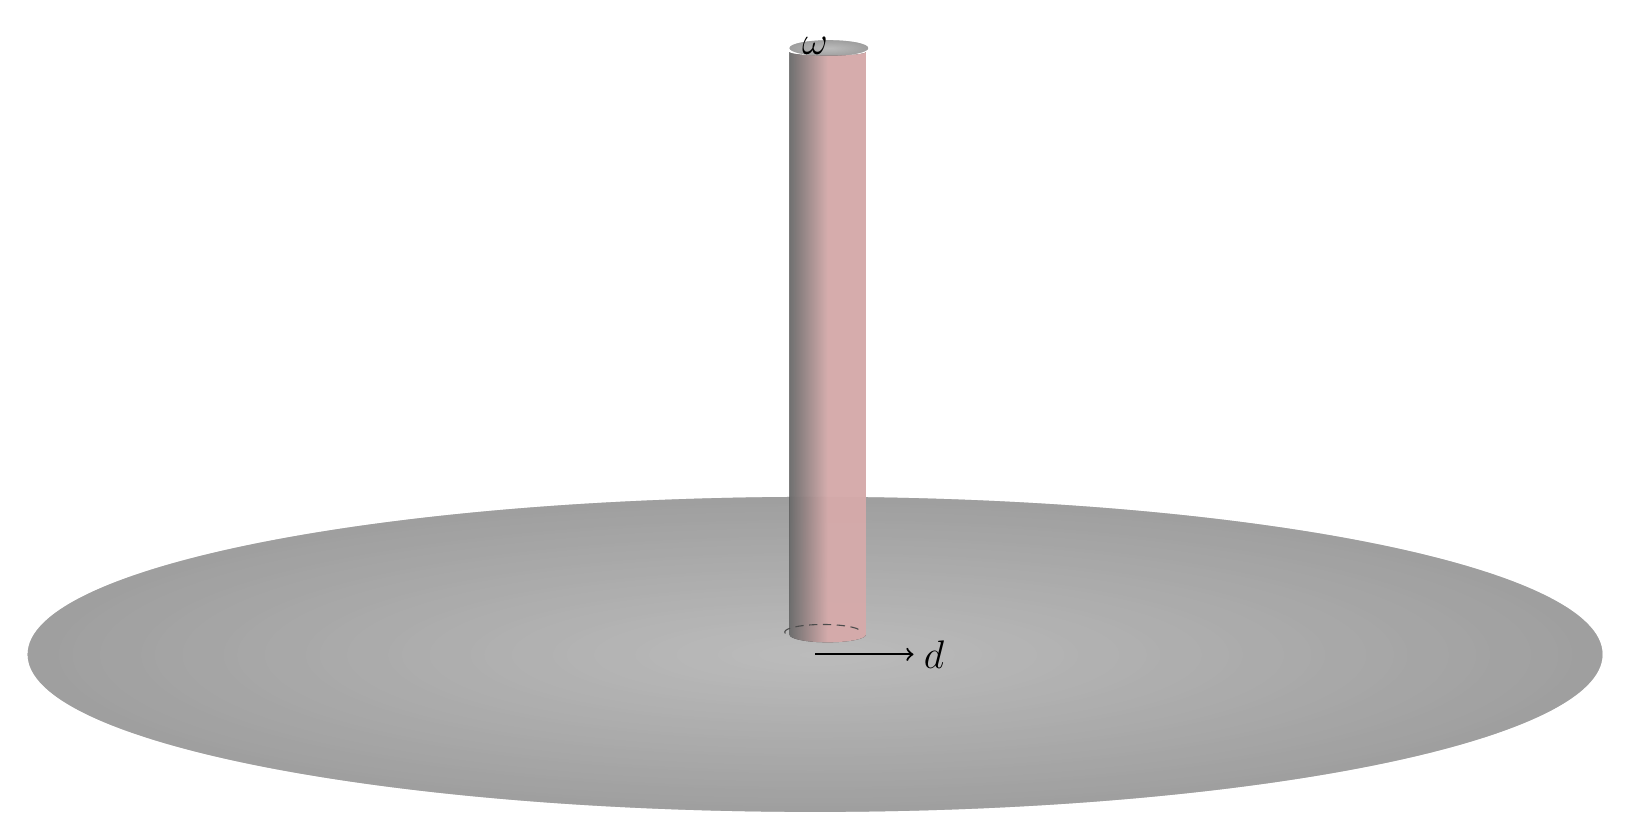
\begin{tikzpicture}[scale=.5]
   %%%%%%%%%%%%%%%%%%%%%%%%%%%%%%%%%%%%%%%%%%%%%%%%
% definitions for schematic
\def\bndmax{5}        %https://tex.stackexchange.com/questions/68462/filling-a-complex-region-with-tikz
\def\bndmin{0.2}
\def \n {20}  % height of y axis
\def \d {12}  % length  of x axis
\def \t {.75}  %  cost of transportation per unit x
\def \th {1}   % theta?
\def \w {15}    %  wage premium
\def \om{1.5}%  omega =rural wage Zero for urban population
\def \azero{2}
\def \aprime {-.0}	
\tikzset{func/.style={thick,color=blue!90}}	

    %%%%%%%%%%%%%%%%%%%%%%%%%%%%%%%%%%%%%%%%%%%%%%%%
% definitions for Cone3
%\node at (0, 2.5){\input{SA_Cone3.tex}};
     \pgfmathsetmacro{\cylinderRadius}{1};%Cone base radius was 9.7
     \pgfmathsetmacro{\coneRadius}{3};%Cone base radius was 9.7
        \pgfmathsetmacro{\coneHeight}{15.1}%Cone height (negative if you want a inverse cone)
           \pgfmathsetmacro{\cylindarHeight}{15.1}%Cone height (negative if you want a inverse cone)
        \pgfmathsetmacro{\cheightp}{.03}%Cut height in percent of cone height

        %Calculating coordinates
        \coordinate (center) at (0,0);
        \pgfmathsetmacro{\MinorAxis}{.2 * \cylinderRadius}; %\  Minor Axis
        \coordinate (peak) at ($(center) + (0,\coneHeight)$);     
        \pgfmathsetmacro{\sradiush}{\cylinderRadius * (1 - \cheightp)};%ADJUST FOR COVERAGE AT CORNERS
        \pgfmathsetmacro{\sradiusv}{.2 * \sradiush};
   %     \pgfmathsetmacro{\sradiusv} {\sradiusv -.1 };

\coordinate (antipeak) at ($(center) + (0,-\coneHeight)$);  %thanks  %I added this
\coordinate (rightB) at ($(center)+(\cylinderRadius,-.2)$);  %vert1-rightB
\coordinate (leftB) at ($(center)-(\cylinderRadius,.2)$);
%problem
\coordinate (svert1) at ($(rightB)!\cheightp!(peak) +(0.1,.75)$);
\coordinate (sleftB) at ($(leftB)!\cheightp!(peak)+(.5,.75)$);  
%. GRID
 %\draw[step=.5,black,thin] (-9.6,0) grid (9.6,7);
 % % Cone Drawing    
%  \fill[ left color=red!70, right colorsradiush cm and \sradiusv cm); 
% ]=red!70,  opacity=20,middle color=red!20,shading=axis] (rightB) -- (peak) -- (sleftB) arc (170:370:\
%    FAT GREEN BAR
%  \draw [fill=green,opacity=80] (-.2, 0) rectangle(.2, \w);
%  \node[above] at (0,\w){$\omega$};
 
%. TOP OF CYLINDER
      \fill[inner color=gray!5,outer color=gray!50,shading=radial,opacity=.5] ($(center) + (.35,.3+\coneHeight)$ ) circle (\cylinderRadius cm and \MinorAxis cm );
      
%  GROUND    
        \fill[inner color=gray!5,outer color=gray!50,shading=radial,opacity=.5] (0,0) circle (20 cm and 4 cm );
      
%        \draw [thick]($(svert1) +(.3,-.3)$)-- ++ (90:\w-.2); % draws vertical lines for edge of cylinder
%        \draw [thick]($(sleftB)-(.2,.3)$)-- ++ (90:\w-.2);
        %Lines, \h in percent of cone height
 def \sradiusv2 \sradiusv cm -.1 cm)
 
% Cylinder drawing  lower left lower right  top right
  \fill[ left color=black!50, right color=red!20,  middle color=red!20, shading=axis, opacity=.8]  (.35 -\cylinderRadius, .5) 
  arc (180:360:\sradiush cm and \sradiusv cm)-- ++(90:\w-.2) 
  arc (360:180:\sradiush cm and \sradiusv2 cm -.1 cm)--cycle;  

   \node[above] at (0,\w){\Large $\omega$};
% TRY TO Make a cylinder
%\draw ($sleftB + (0,\coneHeight)$) [arc (180:360:\sradiush cm and \sradiusv cm)]; 
%     \fill[left color=gray!70,right color=gray!70,middle color=gray!30,shading=axis] (vert1) -- (svert1) arc (0:-180:\sradiush cm and \sradiusv cm) -- (leftB) arc (180:360:\cylinderRadius cm and \MinorAxis cm);

% DASHED LINE AT BACK OF CONE
\foreach \h in {0.03}{   %.38,.34,.30, .7
            \pgfmathsetmacro{\rh}{-\cylinderRadius * (1 - \h)}
            \pgfmathsetmacro{\rv}{.2 * \rh}
            \draw[black!70,densely dashed] ($(sleftB)!\h!(peak)-(.3,.9)$) arc (370:170:\rh cm and \rv cm);%$(leftB)!\h!(peak)$)
        }
        
%  CONE
  %      \draw[opacity=.90, line width=.05cm, green] (0,0)--(0,{\coneHeight - .05});
%     \foreach \h in {0, .38,.34,.30, .7}{
%            \pgfmathsetmacro{\rh}{\cylinderRadius * (1 - \h)} %            \pgfmathsetmacro{\rv}{.2 * \rh}
%            \draw[black!70,densely dashed] ($(antipeak)!\h!(leftB)$) arc (180:360:\rh cm and \rv cm);
%   }
%  \draw[red] (antipeak) arc (30:60:3);
%  \draw[dashed, thick] arc (0:-180:\sradiush cm and \sradiusv cm) -- (leftB) arc (180:360:\cylinderRadius cm and \MinorAxis cm);
%%%%%%%%%%%%%%%%%%%%%%%%%%%%%%%%%

% %\foreach \xi in {0,..., \n} \draw (\xi,0)--(\xi,-.1)node[below=1]{\small$\xi$};
% %\foreach \yi in {1,...,\n} \draw (0,\yi)--(-.1,\yi)node[left]{$\yi$};
% %\foreach \i in {1,4,9,16} {
% %\node at (7,-\om/2){people scattered uniformly across the land  };

% %SECOND FIGURE WITH AGGLOMERATION WAGE
% %  add urban production and net wage
% %\draw[fill=white, white] (0.1,-0.1) rectangle (14,-\om+.1);

% \node[right, text width=4cm] at  (3, \w+1){Added Productivity due to agglomeration};
% %\node[right, text width = 3cm] at  (10,9){Where does the increase in productivity come from?};
 \draw [ thick, ->](0,0)--(2.5, 0)node [right] {\Large $d$};



\end{tikzpicture}




This essay  is written in the classical tradition, making the classical assumption, and asking the classical question. The classics, from Smith to Marx,  all  assumed,  or argued, that an unlimited supply of labour was available at subsistence wages. They then enquired how production grows through time. They found the answer in capital accumulation, which they explained in terms of their analysis of the distribution of income. Classical systems thus determined simultaneously   income distribution and income growth, with the relative prices of commodities as a  minor bye-product.

The purpose of this essay is thus to see what  can be made of the classical  framework  in  solving  problems of distribution, accumulation, and growth, first in a closed and then in an open economy. 



\end{document}